\documentclass{article}

\usepackage{amsmath}
\usepackage{amsfonts}
\usepackage{amssymb}
\usepackage{booktabs}
\usepackage{geometry}
\usepackage{graphicx}
\usepackage{tcolorbox}
\usepackage{tikz}
\usepackage{xcolor}

\usetikzlibrary{arrows.meta, calc, patterns, positioning}

\geometry{a4paper, margin=1in}

\newcommand{\notesetup}[1]{
    \title{#1}
    \author{}
    \date{}
}

\newtcolorbox{keyidea}[1]{
    colback=blue!5,
    colframe=blue!45!black,
    title=#1
}

\newtcolorbox{pitfall}[1]{
    colback=red!4,
    colframe=red!55!black,
    title=#1
}


\begin{document}

\notesetup{Energy and Work}
\maketitle

\section{Why Study Energy?}
Force is not the only useful way to describe motion. In many situations, it is more efficient to track how energy is transferred and transformed.

Examples:
\begin{itemize}
    \item A roller coaster speeds up as it moves downhill.
    \item A moving cart can keep going even after the push stops.
    \item A machine can lift an object to a higher position and store energy in that object.
\end{itemize}

\begin{keyidea}{Core Idea}
Energy is the capacity to do work. Work is the transfer of energy by a force acting through a displacement.
\end{keyidea}

This unit focuses on the first two ideas in a Grade 11 treatment:
\begin{itemize}
    \item identifying forms of energy and describing transformations
    \item calculating work in simple mechanical situations
\end{itemize}

\section{Energy and Energy Transformations}
Energy appears in many different forms. In this unit, we care most about the forms that appear in everyday mechanics problems.

\subsection{Common Forms of Energy}
\begin{itemize}
    \item \textbf{Kinetic energy:} energy of motion
    \item \textbf{Gravitational potential energy:} stored energy due to height
    \item \textbf{Elastic potential energy:} stored energy in stretched or compressed objects
    \item \textbf{Thermal energy:} energy associated with microscopic particle motion
    \item \textbf{Chemical energy:} stored energy in fuels, food, and batteries
\end{itemize}

\subsection{Heat Is Not the Same as Energy Storage}
In physics, \textbf{heat} is energy transferred from a warmer object or region to a cooler one. It is a transfer process, not a separate stored form of mechanical energy.

\subsection{Energy Transformations}
Energy can change from one form to another. For example:
\begin{itemize}
    \item Chemical energy $\rightarrow$ kinetic energy
    \item Gravitational potential energy $\rightarrow$ kinetic energy
    \item Electrical energy $\rightarrow$ thermal energy
    \item Kinetic energy $\rightarrow$ thermal energy + sound
\end{itemize}

It is often helpful to write these as short transformation chains.

\textbf{Example:}
\begin{equation*}
    \text{chemical energy} \rightarrow \text{kinetic energy} \rightarrow \text{thermal energy}
\end{equation*}

\textbf{More examples:}
\begin{itemize}
    \item A falling object: \quad $\text{gravitational potential energy} \rightarrow \text{kinetic energy}$
    \item A car braking: \quad $\text{kinetic energy} \rightarrow \text{thermal energy} + \text{sound}$
    \item A flashlight: \quad $\text{chemical energy} \rightarrow \text{electrical energy} \rightarrow \text{light} + \text{thermal energy}$
\end{itemize}

\subsection{A Useful Habit}
When you read a problem, ask:
\begin{itemize}
    \item What form of energy is present at the start?
    \item What form of energy is present at the end?
    \item Is energy being transferred by work, heat, or both?
\end{itemize}

\subsection*{Sample Problem: Writing an Energy Transformation}
\textbf{Problem:} Describe the main energy transformations when a cyclist brakes to a stop on a level road.

\textbf{Solution:} At the start, the bicycle-rider system has kinetic energy. As the brakes and tires rub, that kinetic energy is transformed mainly into thermal energy, with a small amount into sound.
\begin{equation*}
    \text{kinetic energy} \rightarrow \text{thermal energy} + \text{sound}
\end{equation*}

\begin{pitfall}{Common Mistake}
Students often treat energy as if it disappears. In physics, we usually say the energy is \textbf{transformed} or \textbf{transferred}, not destroyed.
\end{pitfall}

\section{Work ($W$)}
In everyday language, ``work'' can mean effort. In physics, work has a much more specific meaning.

\begin{keyidea}{Definition of Work}
Work is the energy transferred to or from an object by a force acting through a displacement.
\end{keyidea}

\subsection{When the Force and Displacement Are Parallel}
If a constant force acts in the same direction as the displacement, then
\begin{equation}
    W = F \Delta d
\end{equation}

Where:
\begin{itemize}
    \item $W$ is work, measured in joules ($\text{J}$)
    \item $F$ is the magnitude of the applied force, measured in newtons ($\text{N}$)
    \item $\Delta d$ is the magnitude of the displacement, measured in metres ($\text{m}$)
\end{itemize}

Since
\begin{equation*}
    1\,\text{J} = 1\,\text{N}\cdot\text{m}
\end{equation*}
the joule is the SI unit for both work and energy.

\subsection{What This Formula Means}
The amount of work increases when:
\begin{itemize}
    \item the force is larger
    \item the displacement is larger
\end{itemize}

So if you apply twice the force over the same distance, you do twice the work. If you apply the same force over twice the distance, you also do twice the work.

\subsection*{Sample Problem 1: Work by a Constant Force}
\textbf{Problem:} A student pushes a box across the floor with a horizontal force of $35\,\text{N}$. The box moves $4.0\,\text{m}$ in the direction of the force. How much work does the student do on the box?

\textbf{Solution:}
\begin{equation*}
    W = F \Delta d
\end{equation*}
\begin{equation*}
    W = (35)(4.0) = 140\,\text{J}
\end{equation*}

\subsection{Force-Displacement Graphs}
If a force remains constant while an object moves, a force-displacement graph is a useful way to represent the work done.

\begin{figure}[h]
    \centering
    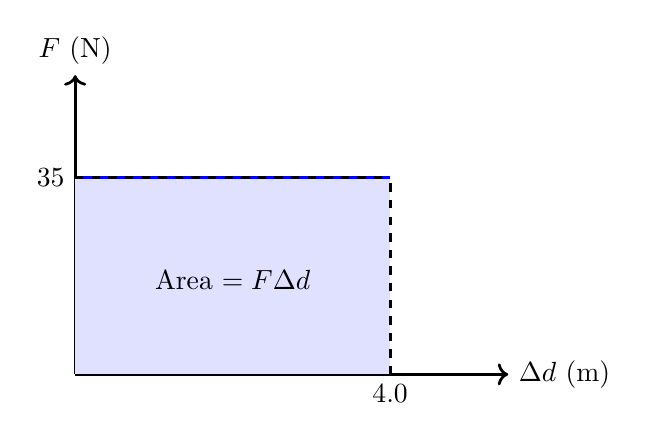
\begin{tikzpicture}[scale=1.0, line width=1pt]
        \draw[->] (0,0) -- (5.5,0) node[right] {$\Delta d\ (\text{m})$};
        \draw[->] (0,0) -- (0,3.8) node[above] {$F\ (\text{N})$};
        \fill[blue!12] (0,0) rectangle (4,2.5);
        \draw[thick, blue] (0,2.5) -- (4,2.5);
        \draw[dashed] (4,0) -- (4,2.5);
        \draw[dashed] (0,2.5) -- (4,2.5);
        \node[left] at (0,2.5) {$35$};
        \node[below] at (4,0) {$4.0$};
        \node at (2,1.2) {Area $= F\Delta d$};
    \end{tikzpicture}
    \caption{For a constant force, the area under an $F-\Delta d$ graph equals the work done.}
\end{figure}

\begin{keyidea}{Graph Meaning}
The area under a force-displacement graph represents the work done by the force.
\end{keyidea}

In the graph above, the area is a rectangle:
\begin{equation*}
    W = (\text{base})(\text{height}) = (4.0\,\text{m})(35\,\text{N}) = 140\,\text{J}
\end{equation*}

So this graph gives the same result as the equation $W = F\Delta d$.

\subsection{When Are You \emph{Not} Doing Work?}
This is one of the most important idea checks in this topic.

\begin{itemize}
    \item If the object does not move, then $\Delta d = 0$, so the work is zero.
    \item If the force is perpendicular to the displacement, then the force does no work.
    \item If there is no force component along the displacement, there is no work.
\end{itemize}

\textbf{Example:} Holding a heavy box while standing still may feel tiring, but in physics you do no work on the box because the box has no displacement.

\subsection{Positive, Negative, and Zero Work}
\begin{itemize}
    \item \textbf{Positive work:} The force and displacement are in the same direction.
    \item \textbf{Negative work:} The force and displacement are in opposite directions.
    \item \textbf{Zero work:} There is no displacement, or the force has no component along the displacement.
\end{itemize}

\textbf{Examples:}
\begin{itemize}
    \item A person pushing a box forward does positive work on the box.
    \item Friction usually does negative work.
    \item Holding a heavy bag still does zero work on the bag because the bag does not move.
    \item A normal force often does zero work because it is perpendicular to the motion.
\end{itemize}

\begin{keyidea}{Sign of Work}
Positive work tends to increase an object's speed. Negative work tends to decrease an object's speed.
\end{keyidea}

\subsection*{Sample Problem 2: Negative Work by Friction}
\textbf{Problem:} A sled moves $12\,\text{m}$ across snow while kinetic friction of magnitude $18\,\text{N}$ acts opposite the motion. What work does friction do on the sled?

\textbf{Solution:}
Because the friction force is opposite the displacement, the work is negative:
\begin{equation*}
    W = -F \Delta d
\end{equation*}
\begin{equation*}
    W = -(18)(12) = -216\,\text{J}
\end{equation*}

\begin{figure}[h]
    \centering
    \begin{minipage}{0.31\textwidth}
        \centering
        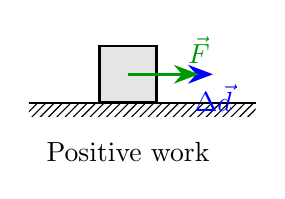
\begin{tikzpicture}[scale=0.9, line width=1pt]
            \draw[thick] (-1.4,0) -- (1.8,0);
            \fill[pattern=north east lines] (-1.4,-0.2) rectangle (1.8,0);
            \draw[fill=gray!20] (-0.4,0) rectangle (0.4,0.8);
            \draw[-{Stealth[scale=1.2]}, blue] (0,0.4) -- (1.2,0.4) node[below] {$\Delta \vec{d}$};
            \draw[-{Stealth[scale=1.2]}, green!60!black] (0,0.4) -- (1.0,0.4) node[above] {$\vec{F}$};
            \node at (0,-0.7) {Positive work};
        \end{tikzpicture}
    \end{minipage}
    \hfill
    \begin{minipage}{0.31\textwidth}
        \centering
        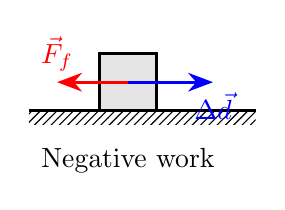
\begin{tikzpicture}[scale=0.9, line width=1pt]
            \draw[thick] (-1.4,0) -- (1.8,0);
            \fill[pattern=north east lines] (-1.4,-0.2) rectangle (1.8,0);
            \draw[fill=gray!20] (-0.4,0) rectangle (0.4,0.8);
            \draw[-{Stealth[scale=1.2]}, blue] (0,0.4) -- (1.2,0.4) node[below] {$\Delta \vec{d}$};
            \draw[-{Stealth[scale=1.2]}, red] (0,0.4) -- (-1.0,0.4) node[above] {$\vec{F}_{f}$};
            \node at (0,-0.7) {Negative work};
        \end{tikzpicture}
    \end{minipage}
    \hfill
    \begin{minipage}{0.31\textwidth}
        \centering
        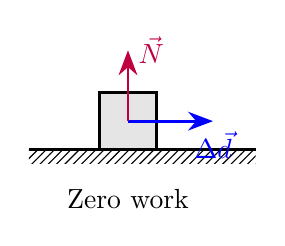
\begin{tikzpicture}[scale=0.9, line width=1pt]
            \draw[thick] (-1.4,0) -- (1.8,0);
            \fill[pattern=north east lines] (-1.4,-0.2) rectangle (1.8,0);
            \draw[fill=gray!20] (-0.4,0) rectangle (0.4,0.8);
            \draw[-{Stealth[scale=1.2]}, blue] (0,0.4) -- (1.2,0.4) node[below] {$\Delta \vec{d}$};
            \draw[-{Stealth[scale=1.2]}, purple] (0,0.4) -- (0,1.4) node[right] {$\vec{N}$};
            \node at (0,-0.7) {Zero work};
        \end{tikzpicture}
    \end{minipage}
    \caption{The sign of work depends on the direction of the force relative to the displacement.}
\end{figure}

\subsection{Work Done Against Gravity}
If you lift an object upward at constant speed, the upward applied force has the same magnitude as the object's weight:
\begin{equation*}
    F = mg
\end{equation*}

So the work done in lifting the object through a vertical height $\Delta h$ is
\begin{equation}
    W = F \Delta h = mg \Delta h
\end{equation}

This idea will be important later when we connect work to gravitational potential energy.

\subsection*{Sample Problem 3: Work Done Lifting an Object}
\textbf{Problem:} A $6.0\,\text{kg}$ backpack is lifted straight upward by $1.4\,\text{m}$ at constant speed. How much work is done by the lifting force?

\textbf{Solution:}
At constant speed, the lifting force equals the weight:
\begin{equation*}
    F = mg = (6.0)(9.8) = 58.8\,\text{N}
\end{equation*}
Then
\begin{equation*}
    W = F \Delta h = (58.8)(1.4) \approx 82\,\text{J}
\end{equation*}

\subsection{Preview: Reference Level}
Later, when we talk about gravitational potential energy, we will need a \textbf{reference level}. This is the level we choose to call zero height. The value of height depends on that choice, but the \textbf{change} in height is what matters most in calculations.

\begin{pitfall}{Common Mistake}
If an object is moving horizontally while gravity acts vertically downward, the work done by gravity is not found using $W = Fd$ directly. You must first decide whether the force has a component along the displacement.
\end{pitfall}

\subsection{Extension: The More General Formula}
For 11th grade, most problems can be handled when force and displacement are parallel or opposite. The more general version is
\begin{equation}
    W = \vec{F} \cdot \Delta \vec{d} = F \Delta d \cos \theta
\end{equation}

Here $\theta$ is the angle between the force and the displacement.

\begin{keyidea}{What the Dot Product Means Physically}
Only the component of force parallel to the displacement does work.
\end{keyidea}

You do \textbf{not} need a full unit on vector multiplication yet. For now, the important idea is simply:
\begin{itemize}
    \item parallel force $\Rightarrow$ maximum work
    \item opposite force $\Rightarrow$ negative work
    \item perpendicular force $\Rightarrow$ zero work
\end{itemize}

\subsection*{Optional Extension Example}
\textbf{Problem:} A person pulls a wagon with a force of $50\,\text{N}$ at an angle of $30^\circ$ above the horizontal. The wagon moves $6.0\,\text{m}$ horizontally. How much work is done by the pulling force?

\textbf{Solution:}
\begin{equation*}
    W = F \Delta d \cos \theta
\end{equation*}
\begin{equation*}
    W = (50)(6.0)\cos 30^\circ \approx 260\,\text{J}
\end{equation*}
Only the horizontal component of the force does work on the wagon.

\section{Quick Concept Check}
\begin{enumerate}
    \item If you push on a wall and the wall does not move, how much work do you do on the wall?
    \item If a box moves to the right and friction acts to the left, is the work done by friction positive or negative?
    \item When a book falls from a desk, which energy transformation is most important: kinetic to gravitational, or gravitational to kinetic?
    \item Why does holding a backpack still on your shoulder do zero work on the backpack?
\end{enumerate}

\section{Summary}
\begin{itemize}
    \item Energy is the capacity to do work.
    \item Heat is energy transferred from a warmer region to a cooler one.
    \item Energy can be transferred and transformed from one form to another.
    \item When force and displacement are parallel, work is given by $W = F \Delta d$.
    \item Positive work tends to increase motion; negative work tends to oppose motion.
    \item Lifting an object through a height $\Delta h$ requires work $W = mg \Delta h$ when the speed is constant.
    \item The general work formula is $W = F \Delta d \cos \theta$.
\end{itemize}

\end{document}
